%%%%%%%%%%%%%%%%%%%%%%%%%%%%%%%%%%%%%%%%%
% Short Sectioned Assignment
% LaTeX Template
% Version 1.0 (5/5/12)
%
% This template has been downloaded from:
% http://www.LaTeXTemplates.com
%
% Original author:
% Frits Wenneker (http://www.howtotex.com)
%
% License:
% CC BY-NC-SA 3.0 (http://creativecommons.org/licenses/by-nc-sa/3.0/)
%
%%%%%%%%%%%%%%%%%%%%%%%%%%%%%%%%%%%%%%%%%

%----------------------------------------------------------------------------------------
%	PACKAGES AND OTHER DOCUMENT CONFIGURATIONS
%----------------------------------------------------------------------------------------

\documentclass[letterpaper, fontsize=11pt]{scrartcl} % A4 paper and 11pt font size

\usepackage[T1]{fontenc} % Use 8-bit encoding that has 256 glyphs
\usepackage{fourier} % Use the Adobe Utopia font for the document - comment this line to return to the LaTeX default
\usepackage[english]{babel} % English language/hyphenation
\usepackage{amsmath,amsfonts,amsthm} % Math packages

\usepackage{lipsum} % Used for inserting dummy 'Lorem ipsum' text into the template
\usepackage[margin=1in]{geometry} %set margins -TA
\usepackage{sectsty} % Allows customizing section commands
\allsectionsfont{\centering \normalfont\scshape} % Make all sections centered, the default font and small caps
\usepackage{enumitem}
\usepackage{fancyhdr} % Custom headers and footers
\usepackage{graphicx}
\pagestyle{fancyplain} % Makes all pages in the document conform to the custom headers and footers
\fancyhead{} % No page header - if you want one, create it in the same way as the footers below
\fancyfoot[L]{\textit{CME 102 Winter '17-'18}} % Empty left footer
\fancyfoot[C]{} % Empty center footer
\fancyfoot[R]{Tim Anderson} % Page numbering for right footer
\renewcommand{\headrulewidth}{0pt} % Remove header underlines
\renewcommand{\footrulewidth}{0pt} % Remove footer underlines
\setlength{\headheight}{14pt} % Customize the height of the header

\numberwithin{equation}{section} % Number equations within sections (i.e. 1.1, 1.2, 2.1, 2.2 instead of 1, 2, 3, 4)
\numberwithin{figure}{section} % Number figures within sections (i.e. 1.1, 1.2, 2.1, 2.2 instead of 1, 2, 3, 4)
\numberwithin{table}{section} % Number tables within sections (i.e. 1.1, 1.2, 2.1, 2.2 instead of 1, 2, 3, 4)

\setlength\parindent{0pt} % Removes all indentation from paragraphs - comment this line for an assignment with lots of text
\begin{document}

%----------------------------------------------------------------------------------------
%	TITLE SECTION
%----------------------------------------------------------------------------------------

\newcommand{\horrule}[1]{\rule{\linewidth}{#1}} % Create horizontal rule command with 1 argument of height

%----------------------------------------------------------------------------------------
%	PROBLEM 1
%----------------------------------------------------------------------------------------

\section*{Week 8 Section Problems}
\par If not otherwise specified, solve the following problems. If initial conditions are given, solve for all constants of integration. It is okay to leave answers in implicit form or with unsolved integrals. 
\begin{enumerate}
\item For the following, give the natural frequency \textit{$\omega_0$}. State whether or not there is resonance or beats, and give a reason for why.
\begin{enumerate}
\item $y'' + 4y = sin(2t)$
\item $y'' + 5y' + 2y = cos(2t)$
\item $y'' + y' + 2y = 3$
\item $y'' + 4y = sin(2.05t)$
\end{enumerate}

\item For the system described by the image below, derive the system of ODEs governing the mass-spring system. Treat the masses as point masses and assume no damping or friction.
\newline
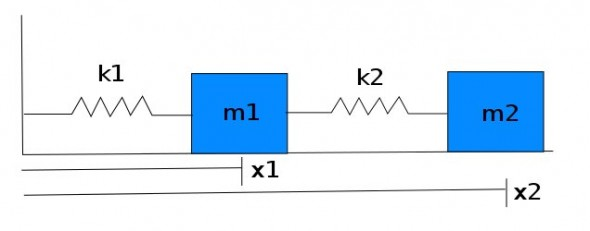
\includegraphics[width=5in]{section8_1.jpg}

\item Perform the following integrals:
\begin{enumerate}
\item $\int_{0}^{\infty}e^{-sx} dx$
\item $\int_{0}^{\infty}sin(x)e^{-sx} dx$
\item $\int_{0}^{\infty}u(x-2)sin(x-2)e^{-sx} dx$
\end{enumerate}

\item Solve the following using a Laplace transform: $$y'' - 2y' + y = 2 \; ; \qquad y(0) = 0 \qquad y'(0) = 0$$


\end{enumerate}

%----------------------------------------------------------------------------------------

\end{document}